\subsection{Table Tennis}

\begin{enumerate}

\begin{figure}[htbp] % htbp are float placement options
\centering
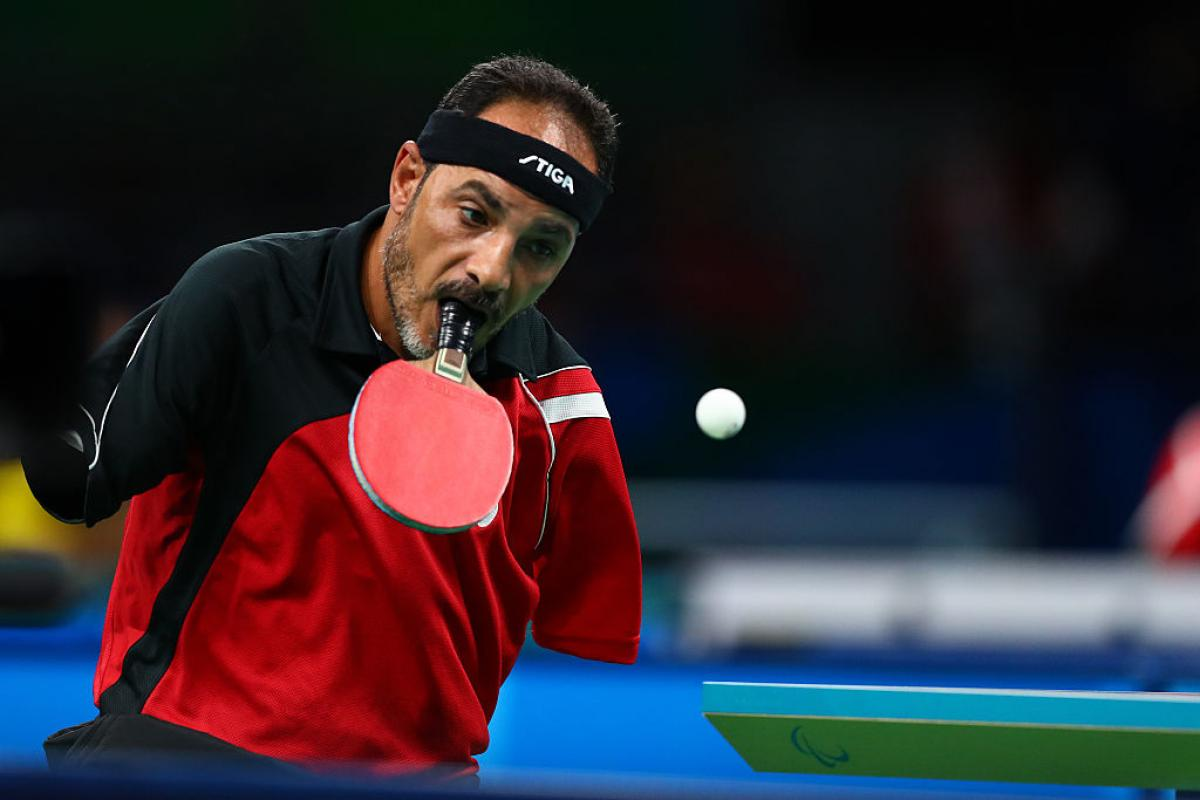
\includegraphics[width=0.8\textwidth]{Images/para_tabletennis.jpg}
\caption{Para Tabletennis}
\label{fig:my_image}
\end{figure}

\item Essence of Table Tennis
    \begin{itemize}
    \item Paralympic table tennis is a fast-paced and exhilarating sport that showcases the agility, reflexes, and tactical brilliance of athletes with various impairments. 
    \item Players compete in standing or wheelchair categories, battling each other across a table with small rackets and a lightweight ball. 
    \item The sport demands lightning-fast reactions, precise hand-eye coordination, and strategic shot placement, captivating spectators with its intensity and skill.
    \end{itemize}

\item Rules, Equipment, and Competition
    \begin{itemize}
    \item Paralympic table tennis adheres to the fundamental rules of table tennis, with adaptations made to accommodate different impairments. 
    \item The game is played in singles and doubles formats, and points are scored by hitting the ball onto the opponent's side of the table so that they cannot return it legally. 
    \item The sport utilizes a standard table tennis table, net, and balls, and athletes can use adaptive equipment like wheelchairs or prosthetic limbs based on their classification.
    \end{itemize}

\item Categories and Classifications
    \begin{itemize}
    \item Paralympic table tennis employs a classification system that groups athletes based on the impact of their impairment on their playing ability. 
    \item Athletes are categorized into different classes, with classes 1-5 for wheelchair users and classes 6-10 for standing players. 
    \item The classifications consider factors such as muscle power, range of movement, and balance, ensuring fair competition among athletes with similar functional abilities.
    \end{itemize}

\end{enumerate}